\documentclass[10pt]{article}
\usepackage{color, natbib, graphicx}
\usepackage{dsc2003}

\begin{document}

\title{Visualizing the independence problem using extended association and
mosaic plots}
\author{David Meyer
\thanks{Institute of Statistics and Probability Theory, Vienna University of Technology}
\And
Achim Zeileis 
\thanks{Institute of Statistics and Probability Theory, Vienna
University of Technology}
\And
Kurt Hornik
\thanks{Institute of Statistics, Vienna
University of Economics and Business Administration}
}

\maketitle

\section{Introduction}

Statistical models built for the analysis of multivariate data,
quickly become complex with increasing dimensionality.
One idea of visualization techniques is to
use the human visual system to detect structures in the data that
possibly are not obvious from solely numeric output (e.g., test
statistics).
The {\sf R} package `\texttt{vcd}'---based on the Book `Visualizing Categorical
Data' \cite[][]{vcd:Friendly:2000}---includes methods for the (mostly
graphical) exploration of categorical data, such as:
\begin{itemize}
 \item fitting and graphing of discrete data,
 \item plots for the independence and symmetry problems, and
 \item visualization techniques for log-linear models.
\end{itemize}
In this talk, we focus on the visualization of the independence
problem, typically analyzed using a table of relative frequencies $\pi_{ij\dots}$
with two or more dimensions. In the setting of bivariate problems, the
null hypotheses is $\pi_{ij} = \pi_{i+}\pi_{+j}$. With additional variables
(often used to stratify the data), more independence models can be
envisaged, including the null hypotheses of:
\begin{itemize}
 \item total independence:
  $\pi_{ijk\dots} = \pi_{i++\dots}\pi_{+j+\dots}\pi_{++k\dots}\dots$
 \item conditional independence:
  $\pi_{ijk\dots} = \pi_{i|k\dots}\pi_{j|k\dots}$
 \item joint independence:
  $\pi_{ijk\dots} = \pi_{ij+\dots}\pi_{++k\dots}$
\end{itemize}
Classical non-graphical methods for these problems include the Chi-square
test, Fisher's exact test (for fourfold tables), the
Cochran-Mantel-Haenzel test (for $2 \times 2 \times
n$-tables), and the analysis of log-linear models for more
complex settings.
    
\section{Association Plots}

Association plots \cite[][]{vcd:Cohen:1980} are inspired by the classical Chi-squared test of
independence for two categorical variables, which---based on a $m
\times n$-table of observed frequencies $o_{ij}$---is performed using the test
statistic

\[\chi^2 = \sum_{i}^{m}\sum_{j}^{n}r_{ij}^2\]

\noindent where the \emph{Pearson-residuals} $r_{ij}$ are the standardized deviations
of the observed from the expected frequencies:

\[r_{ij} = \frac{o_{ij} - e_{ij}}{\sqrt{e_{ij}}}\]

\noindent Under the null of independence, $e_{ij} = o_{i+}o_{+j}/o_{++}$, and $\chi^2$
follows a Chi-squared distribution with $(m-1)(n-1)$ degrees of
freedom.

The association plot precisely visualizes the table of
Pearson-residuals (see Figure \ref{fig:assocbase}):
each cell is represented by a rectangle that has (signed) height
proportional to the corresponding Pearson-residual $r_{ij}$ and width proportional to the
square root of the expected counts $\sqrt{e_{ij}}$. Thus the area is proportional to
the raw residuals $o_{ij} - e_{ij}$. The sign of the residual is redundantly
coded by orientation and color of the corresponding rectangle.

\begin{figure*}[htbp]
  \begin{center}
    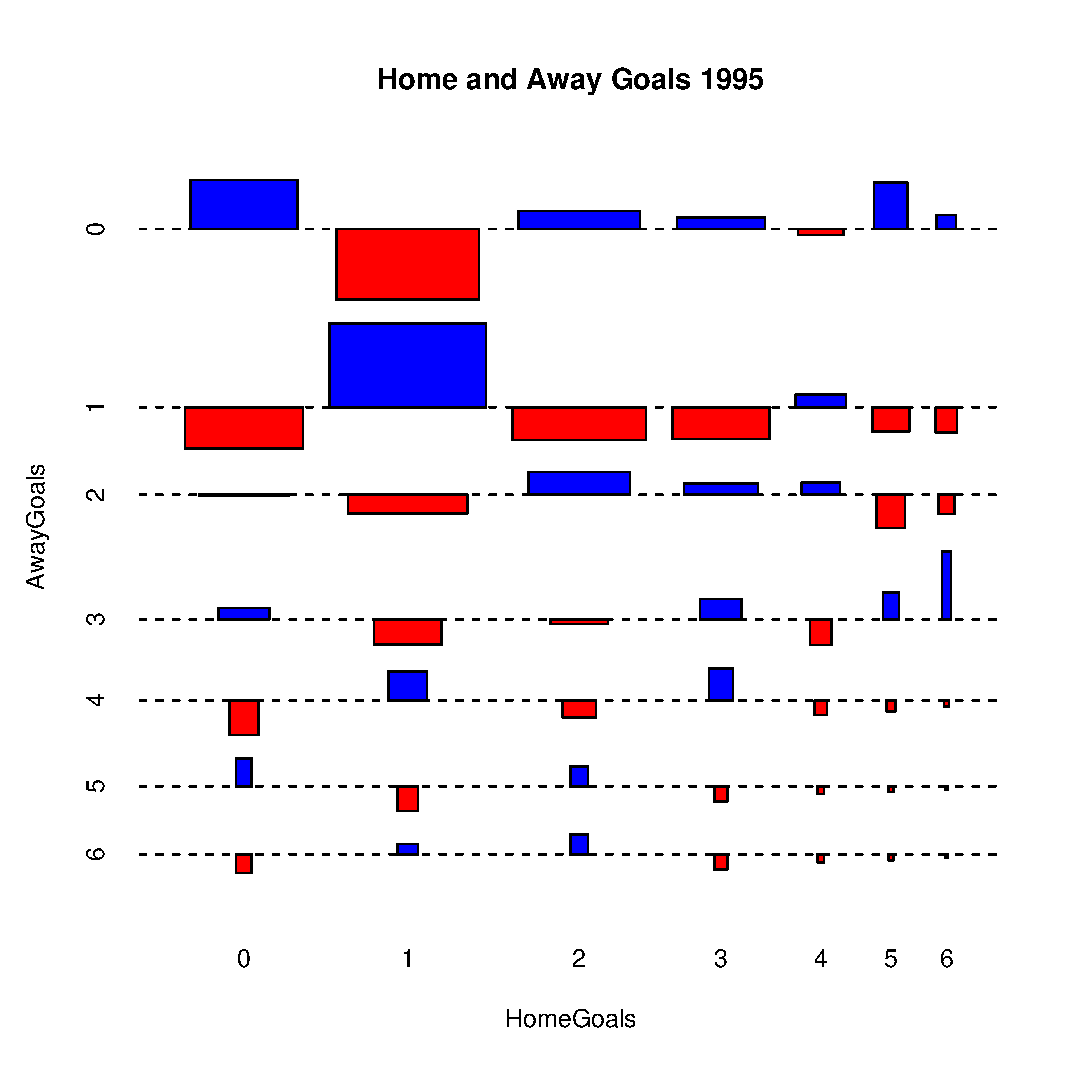
\includegraphics[width = 10cm]{assocbase}
    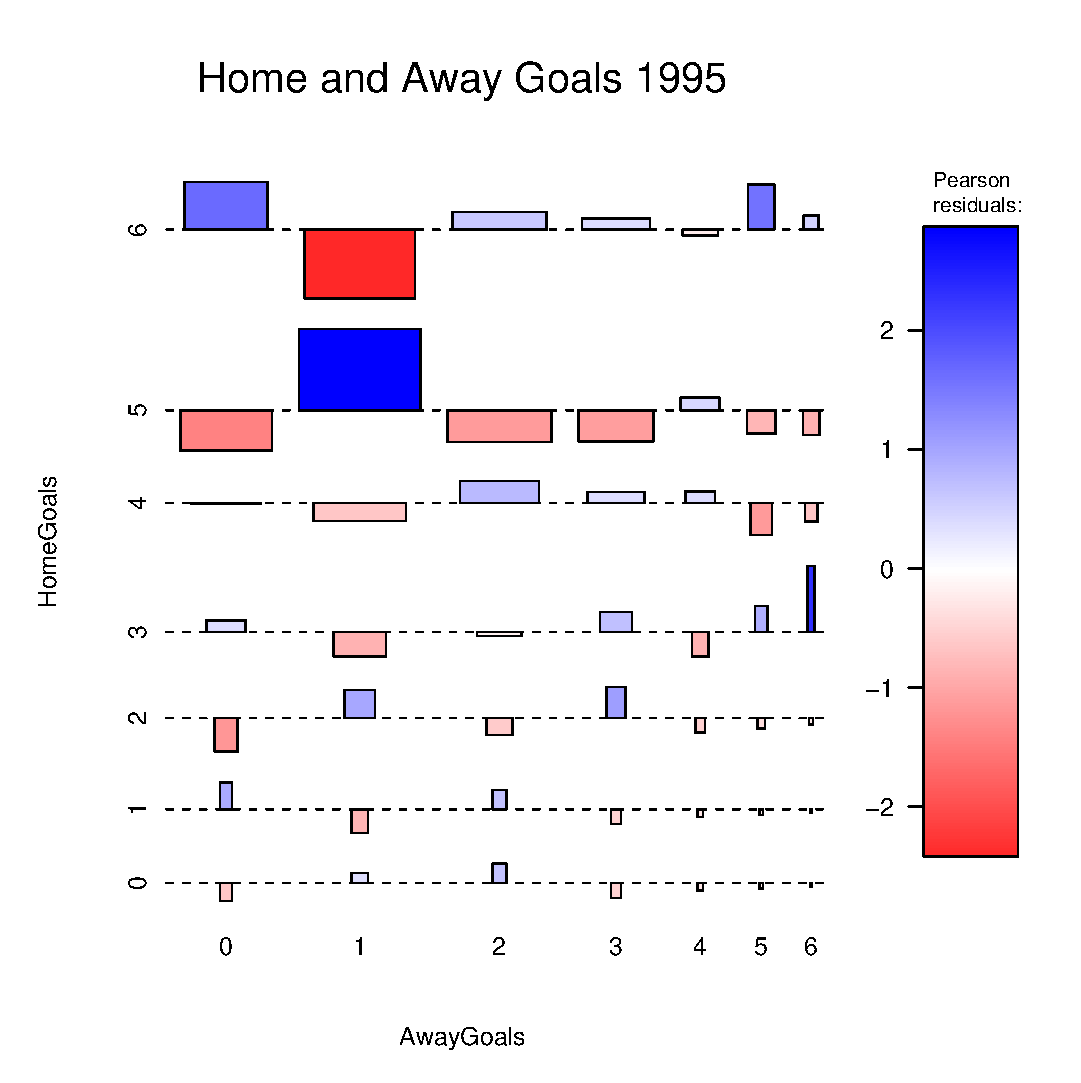
\includegraphics[width = 10cm]{assocnew}
    \caption{`Classical' (top) and extended (bottom) association plot
    for the 1995 home and away goals of the Deutsche Bundesliga. The
    shading gives more information on the importance of the Pearson residuals.}
    \label{fig:assocbase}
  \end{center}
\end{figure*}

% [1 graphisches Beispiel; HairEyeColor? Fussballdaten?]
        
\section{Mosaic Plots}
Mosaic Plots can be seen as an extension of grouped
bar charts, where width and heights of the bars show the relative
frequencies of the two variables: a mosaic plot simply
consists of a collection of tiles whose
sizes are proportional to the observed cell frequencies (see Figure \ref{fig:mosaicbase}).

\begin{figure*}[htbp]
  \begin{center}
    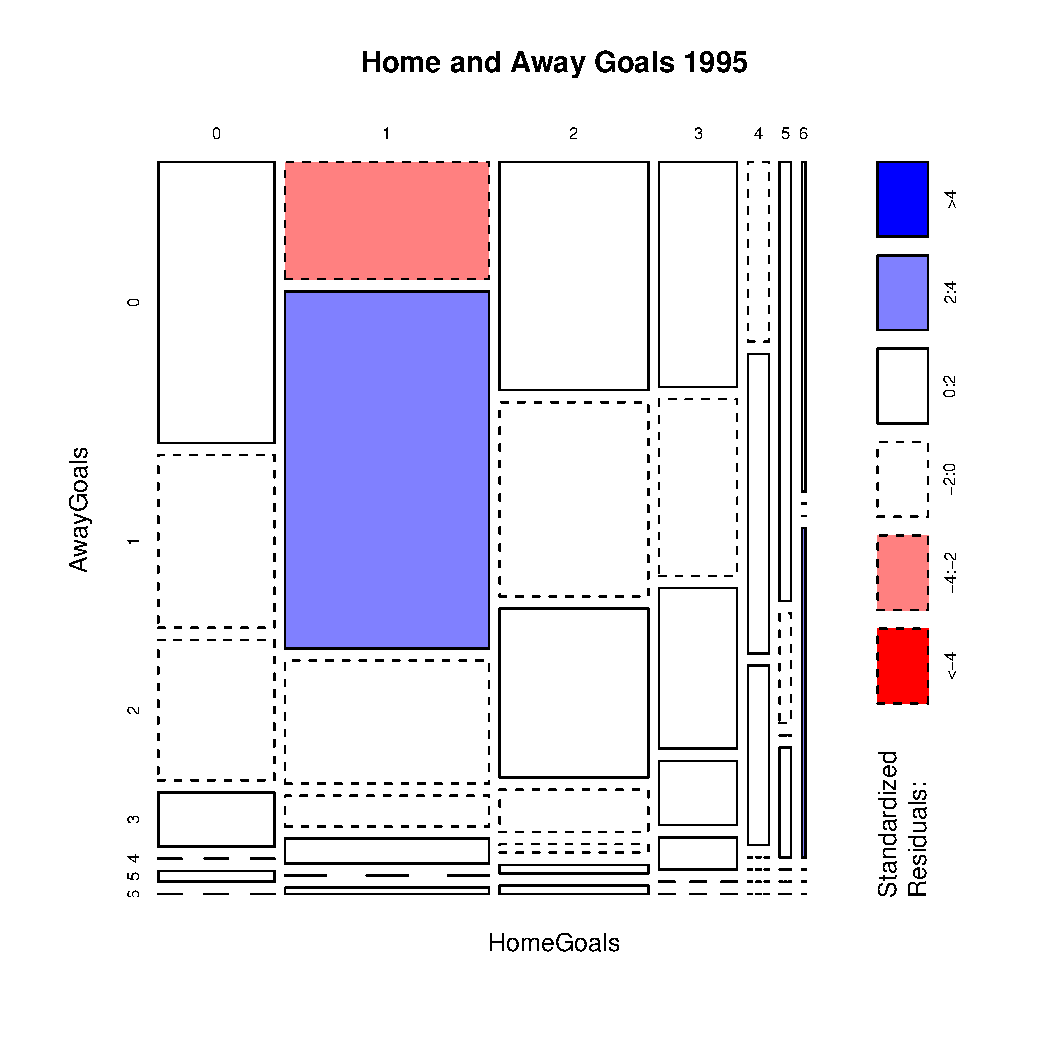
\includegraphics[width = 10cm]{mosaicbase}
    \caption{Mosaic plot (with Friendly extensions)
    for the 1995 home and away goals of the Deutsche Bundesliga. As in
    extended association plots, the shading visualizes the deviations
    (residuals) from the independence model.}
    \label{fig:mosaicbase}
  \end{center}
\end{figure*}

Sequential horizontal and vertical recursive splits are used to
visualize the frequencies of more than 2 variables, each new variable
conditional to the previously entered variables. A first extension by
\cite[][]{vcd:Friendly:1994} uses a color coding of the tiles to visualize deviations
(residuals) from a given log-linear model fitted to the table, that is, from
the expected frequencies under arbitrary (independence)
hypotheses---the color of each tile depending on the sign, and the
brightness being proportional to the corresponding residual.

% [1 graphisches Beispiel mit selben Daten]
        
\section{Extensions}
Our extensions to these two visualization methods cover three topics:
improvement of color coding, visualization of the overall
test of independence, and flexible specification of graphical
parameters.
The color schemes used by Michael Friendly in his implementations are
rather poor, due to limitations of the SAS software used that only
implements a discrete color palette in the `RGB' color space that does not, e.g., 
allow for copier proofness and homogeneous saturations over different colors. Our
implementation uses continuous color schemes in the device-independent
`HCL' (Hue-Chroma-Luminance) color space. The continuous scheme is
more appropriate to visualize the importance of the Pearson residuals
as any possible discretization of the scale.

In addition to the `local' independence information (shading of the
residuals), we also offer to simultaneously visualize the overall independence
model by adding white stripes to the rectangles as long as a specified test does not
reject the null---the colors, then, appear `lighter' than without stripes.
The user currently can choose the test---either the classical
Chi-Square test, or the maximum-residual test. The latter uses a
(sampled) conditional exact distribution of the maximal Pearson
residual (compared to the sum of squared residuals used for the
Chi-squared test). Using this maximum-test assures consistency between the `local' and
`global' independence information: when the overall model is
significant, the plot indeed visualizes the `guilty' residuals.

Finally, one might wish to use graphical parameters varying from tile
to tile to visualize additional information.
Our implementation offers full control over 
each element by using a call-back function
invoked each time a tile is plotted and that is given the position
information (that is, the index in the visualized table).

\section{Conclusion}
Both methods described (association plot and mosaic plot) are used to
visualize the independence problem. Our extensions include better
color schemes, visualization of the overall independence model, and
more flexible manipulation of the graphical parameters.
Future Work will include extensions for more than two dimensions
(such as conditional plots or trellis layouts), and improved
labelling.

\bibliographystyle{apalike}
\bibliography{vcd}

\end{document}
% LocalWords:  proofness

